\documentclass[11pt]{article}
%\usepackage{authblk}
\usepackage[titletoc,page]{appendix}
\usepackage{titling}
	\addtolength{\oddsidemargin}{-.875in}
	\addtolength{\evensidemargin}{-.875in}
	\addtolength{\textwidth}{1.75in}
	\addtolength{\topmargin}{-.875in}
	\addtolength{\textheight}{1.75in}
\usepackage{indentfirst}



\title{Checkpoint Report\\
\large On the Implementation of the Emulator \\
       for the Assessed C Laboratory Project}
      
     
\author{
    Izabella Kacprzak\\
    Matthew Hill
    \and 
    Nicole Obretincheva\\
    \'Una Miralles}


\date{June 5, 2020}

\usepackage{natbib}
\usepackage{graphicx}

\begin{document}

\maketitle



\section{Group Organisation}
The core functions of the emulator, such as instruction fetching, pipeline management and the fetch decode execute loop, were implemented as a collective to make sure every team member was aware of the core operation and structure of the program. Someone would code up the solution whilst sharing their screen via a video conference application such as Microsoft Teams™ so that other group members can spot their mistakes. This meant that we were clear on the input to and output from the functions that we wrote when we split up.\\ 
\indent Individual group members were assigned to complete simple functions such as loading instructions to memory, printing the output, checking and setting conditional codes, determining an instruction’s type and loading the correct execute function for the instruction type. We then split into teams of two based on time zone differences, with Matthew and Úna handling data processing instructions and Nicole and Izabella handling multiply, single data transfer and branch instructions as data processing was much more complicated and needed lots of auxiliary helper functions. The offset calculation was the same in both the single data transfer and data processing instructions so we decided that the group that implemented data processing would create a function to calculate the offset that was called in both instruction functions, preventing code duplication.\\
\indent We met in the mornings to merge the git branches we had created whenever we had split work so every group member was present when we merged. These meetings were also used as an opportunity to reassign tasks and to check on everyone’s progress. We also often assigned someone the task of cleaning up code, adding in comments and renaming variables throughout the coding process to improve code consistency and readability.


\section{Group Collaboration}
We think the group worked together well and we divided work fairly. The teams had roughly equal workloads and finished in similar times so no one was left waiting around. The use of paired programming was effective, reducing the frequency of bugs and ensuring collaboration and consistency. However, we think we could have been more effective in integration testing once we recombined the code from the two teams as we found debugging very difficult when trying to pass entire system tests such as the loop or factorial programs, struggling to isolate the errors. We also tried to test the code on everyone’s devices to ensure portability, and in one case this caught an instance of undefined behaviour as an if statement was being entered on everyone’s computer’s but Matthew’s.\\    
\newpage The scheduled meetings with the team were very helpful as that ensured everyone was on the same page and had at least a basic understanding of each function and the way it works resulting in consistent code. Using these meetings to merge git branches was also useful as it meant no key code was accidentally omitted and everyone knew if they were up to date with the master branch. However, \'Una and Matthew often had unreliable Internet connections which lead to the stream freezing or lagging on their perspectives. This lead to difficulties in debugging and communicating with the team. This process was also significantly slower than the pair programming as a result and we often had long programming sessions without breaks which lead to tiredness, especially for Nicole who was working in BST+2 so often was working late at night. Tiredness often leads to careless mistakes in programming and on many occasions we accidentally introduced undefined behaviour which lead to debugging difficulties. Overall, the group collaborated well but we need to improve our methods to be faster and more reliable if someone has technical issues. 


\section{Implementation Strategy}
Our implementation has an emulate file that contains the fetch execute cycle and a function for loading instructions from a file to memory. The fetch execute cycle references functions from a library split into two halves, pipeline utils (for fetching and decoding instructions) and execute utils (for executing instructions). The file structure for the implementation can be seen in Appendix A.
The pipeline utils files contain typedefs for register contents and instructions as well as two structs, one for the machine state and one for the pipeline state, and two enums for instruction types and conditional codes (such as eq). The functions in this file print the output of the program on termination, fetch an instruction and update the pipeline struct, determine the type of an instruction, check if an instruction meets its execution condition and set the CPSR flags. The execute utils files contain a struct representing a data processing operator, an enum for flags, and two public functions for getting a register pointer from an instruction at a start int and for executing an instruction given its type and the machine state. \\
\indent There are many parts of code that could be directly reused in writing the assembler such as the instruction type, flags and conditional code enums. The execute function could be reused in a completely different context as well, calling binary translation functions for each instruction type. In addition, the typedefs for registers and instructions will be useful. There are many other techniques that we have employed that could be used in the assembler in reverse. For example the algorithm for determining types could have its logic reversed to set relevant bits based on a type enum and the offset from register algorithm could be reversed to get the binary sequence that corresponds to a given offset.


\section{Expected Future Difficulties}
For the assembler we may need to re-examine our methods of group collaboration as we will be short of time if we want to complete a substantial extension as well. This means we may need to assign just one person to merge to master and use merge requests instead of merging as a collective and we should split into teams more often rather than coding together. This could lead to problems of more bugs emerging and a lower code understanding so we will have to be really careful when coding and should still meet to explain the choices we have made in implementing our code. In addition, we will have to make changes to the file structure as there are common parts, such as instruction type enums, in both the assembler and emulator so we will need to create a common library between both. To fix this, we have edited the library to have a combined utils file that could be used by both programs to reduce duplication.

\appendix{}
\section{Implementation Diagram}
\begin{figure}[h!]
\centering
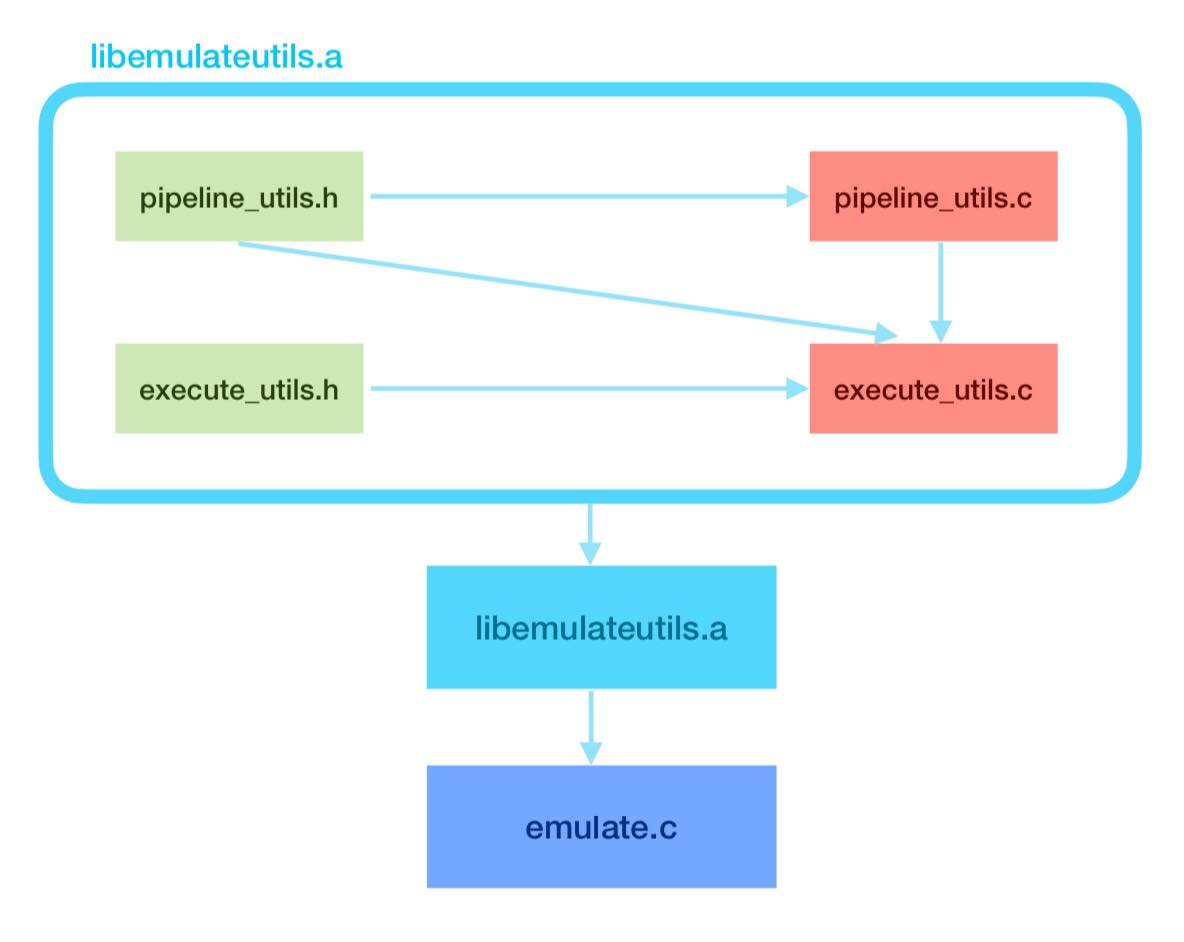
\includegraphics[scale=0.3]{diagram.jpg}
\caption{File Structure}
\end{figure}


\end{document}
